\documentclass[captions=tableheading,parskip=half, bibliography=totoc]{scrartcl} % KOMA-Script Dokumentenklasse Article [titlepage=firstiscover]

% UTF8 input encoding support
\usepackage[utf8]{inputenc}

% scrhack
\usepackage{scrhack}

% Warnung, falls noch einmal kompiliert werden muss
\usepackage[aux]{rerunfilecheck}

% Paket für Schriftarteinstellung, muss immer geladen werden
\usepackage{fontspec}

% Deutsche Spracheinstellungen, wichtig z. B. für korrekte Trennung
\usepackage[main=ngerman]{babel}
\usepackage[autostyle]{csquotes}

\usepackage{ragged2e}
\usepackage{pdfpages}
\usepackage{pdflscape}
\usepackage{rotating}

% adds Blindtext
\usepackage{blindtext}
\usepackage{longtable}

% Math and Science extensions
\usepackage{amsmath, nccmath}
\usepackage{amssymb}
\usepackage{mathtools}
\DeclarePairedDelimiter\abs{\lvert \,}{\rvert}
\DeclarePairedDelimiter{\bra}{\langle}{\rvert}
\DeclarePairedDelimiter{\ket}{\lvert}{\rangle}
\DeclarePairedDelimiterX{\braket}[2]{\langle}{\rangle}{
    #1 \delimsize| #2
    }

\usepackage[math-style=ISO,bold-style=ISO,sans-style=italic,nabla=upright,partial=upright]{unicode-math}
\usepackage[locale=DE, uncertainty-mode = separate]{siunitx}  %[per-mode=symbol-or-fraction]
\sisetup{math-micro=\text{$\symup{\mu}$},text-micro=$\symup{\mu}$}
\usepackage[version=4, math-greek=default, text-greek=default]{mhchem}
\DeclareSIUnit\Div{DIV}
%
\usepackage{graphicx}
\usepackage{grffile}
\usepackage{float}
\floatplacement{figure}{htbp}
\usepackage[labelfont=bf]{caption}
\usepackage[width=0.75\textwidth]{subcaption}

% Bibliography extensions
\usepackage{booktabs}
\usepackage[backend=biber]{biblatex}
\addbibresource{../lit.bib}

\usepackage{microtype}
\usepackage{xfrac}
\usepackage[shortcuts]{extdash}
\usepackage{expl3}
\usepackage{xparse}
\usepackage{mleftright}
\usepackage[shortcuts]{extdash}

\NewDocumentCommand \delnachdel {mm}
{
    \mathinner{\frac{\partial #1}{\partial #2}}
}
\NewDocumentCommand \delnachdelsq {mm}
{
    \mathinner{\frac{\partial^2 #1}{\partial #2 ^2}}
}
\NewDocumentCommand \dnachd {mm}
{
    \mathinner{\frac{\symup{d} #1}{\symup{d} #2}}
}

\NewDocumentCommand \deln {mmm}
{
    \mathinner{\frac{\partial^#3 #1}{\partial #2 ^#3}}
}

\NewDocumentCommand \leftside {m}
{
\flushleft{#1\;}\justifying
}


\NewDocumentCommand \dif {m}
{
    \,\mathinner{\symup{d} #1}
}

\NewDocumentCommand \zz {}
{
    \mathinner{\mathrm{Z\kern-.3em\raise-0.5ex\hbox{Z}}}
}

\ExplSyntaxOff

% Zum Ausschwärzen von Texten

\usepackage{censor}



% Unterstützung für Links und PDF Metadaten
\usepackage[unicode,pdfusetitle]{hyperref}
\usepackage{bookmark}

%\setmathfont{XITS Math}[range={scr,bfcal}]
%\setmathfont{XITS Math}[range={cal,bfcal}, StylisticSet=1]
\sisetup{math-micro=\text{\mu},text-micro=\mu}

\begin{document}
    \pagenumbering{roman}

    \vspace{2cm}
    
    \title{V53 Mikrowellen auf Hohlleitern}
    
    \vspace{1cm}
    
    \author{
        \censor{Luca Di Bella}\\
        \texorpdfstring{\censor{luca.dibella@tu-dortmund.de}\and}{,}
        Tobias Rücker\\
        \texorpdfstring{\href{mailto:tobias.ruecker@tu-dortmund.de}{tobias.ruecker@tu-dortmund.de}}{}
    }
    
    \vspace{1cm}
    
    \date{Durchführung: 10.05.2021 \\ Abgabe: 23.06.2021\vspace{-4ex}}
    
    \maketitle
    \thispagestyle{empty}
    
    \begin{center}
        Versuchsgruppe: \textbf{6}
    \end{center}
    
    \vfill
    
    \begin{center}
        Technische Universität Dortmund\\
        Fortgeschrittenenpraktikum Physik
    \end{center}
    
    \newpage
    \justifying
    \tableofcontents
    \newpage
    \pagenumbering{arabic}
    \clearpage
    \setcounter{page}{1}

% -- Zielsetzung -- %
    \section*{Zielsetzung}
    \addcontentsline{toc}{section}{Zielsetzung}
    In diesem Versuch werden die Eigenschaften von Mikrowellen auf Hohlleitern, welche durch ein Reflexklystron erzeugt werden, untersucht.
    Dabei werden die Wellenlänge und Frequenz bestimmt und das Stehwellenverhältnis  in Abhängigkeit von verschieden starken Störstellen des Hohlleiters ermittelt.
    
%
% -- Theorie -- %
%
    \section{Theorie}
        \subsection{Mikrowellen}
            Mikrowellen sind elektromagnetische Wellen (kurz: EM-Wellen) in einem Frequenzbereich von $\SI{300}{\mega\hertz}$ bis $\SI{300}{\giga\hertz}$,
            welches einen Wellenlängenbereich von $\SI{1}{\meter}$ bis $\SI{30}{\milli\meter}$ umfasst.            
            Hierbei werden zwischen verschiedenen Frequenzbändern unterschieden. In diesem Versuch werden Mikrowellen mit einer Frequenz von ca. $\SI{9}{\giga\hertz}$ untersucht.
            
            Geschichtlich sind Mikrowellen in der Zeit des zweiten Weltkrieges von Herrn Boot und Randall bei der Entwicklung von Sendern für Radaranlagen genutzt worden.
            Die Erzeugung erfolgte dabei über ein Magnetron, eine Vakuum-Laufzeitröhre. Später führte die Forschung des Wissenschaftlers Percy Spencer an dem Magnetron zufällig zur
            Entwicklung und Produktion der ersten kommerziellen Mikrowelle. Andere Arten von Vakuum-Röhren für die Erzeugung 
            von Mikrowellen bilden die Wanderfeldröhre, das Gyrotron und das Klystron.
            
            Trotz der Vorteile von der Mikrowellenstrahlung bietet diese bei direkter Aussetzung
            die Gefahr auf irreparable Schäden für den Menschen. Ein Beispiel bildet hierbei der Fall von den militärischen
            Radaranlagen der Bundeswehr. Bei diesen waren Soldaten und Zivilangestellte der Bundeswehr zwischen 1950 und 1980 den Radaranlagen, welche
            Röntgen- und Mikrowellenstrahlung aussanden, ausgesetzt. Infolgedessen entwickelten mehrere Soldaten Krankheiten wie Krebs und körperliche Behinderungen,
            welche auch auf Kinder von ehemaligen Radarsoldaten vererbt wurden. 
            
        \subsection{Hohlleiter}
            Ein wichtiges Bauteil für die Messung von Mikrowellen stellt der Hohlleiter dar.
            Dieser besteht aus gut elektrisch leitenden Wänden und kann in verschiedenen Formen wie elliptisch, kreisförmig oder rechteckig sein. 
            Je nach Bauart können die Hohlleiter verschiedene Arten von EM-Wellen, genannt Moden, leiten, wobei die Hohlleiter häufig so gebaut werden,
            dass nur die niedrigste Mode des Frequenzbereichs transportiert.\\
            Jeder Hohlleiter besitzt dabei eine Grenzfrequenz unterhalb der keine Energie transferiert werden kann.
            Für einen rechteckigen Hohlleiter der Breite $a$ und Höhe $b$ ergibt sich die Grenzwellenlänge $\lambda_G$ einer transversalen elektrischen Welle (kurz: TE-Welle) $\text{TE}_{n,m}$ rechnerisch aus
            \begin{align}
                \lambda _G &=  \frac{2}{\sqrt{\frac{n^2}{a^2}+\frac{m^2}{b^2}}} \text{\cite{Mikro}} \label{eq:G}
            \end{align}
            wobei $c$ die Lichtgeschwindigkeit im Vakuum ist und $n$ und $m$ zwei Ordnungsparameter sind.


        \subsection{Erzeugung von Mikrowellen: das Reflexklystron}\label{ssec:1.3}
            Es bieten sich verschiedene Möglichkeiten an, um Mikrowellen verschiedener Frequenzbänder oder Intensitäten zu erzeugen.
            Für diesen Versuch wird ein Reflexklystron verwendet.
            \begin{figure}[H]
                \centering
                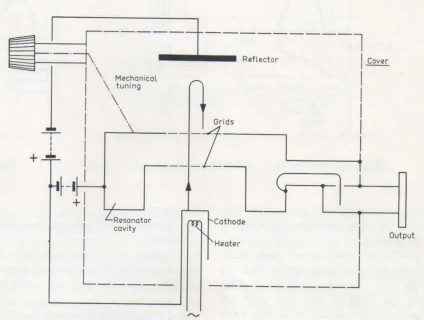
\includegraphics[width=0.6\textwidth]{pics/klystron.jpg}
                \caption{
                    Die Abbildung zeigt den theoretischen Aufbau eines Klystrons.
                    Dieser besteht aus einer Glühkathode, einem Beschleunigungsgitter,
                    einem Hohlraumresonator und einem Reflektor. Die Funktionsweise wird in Abschnitt \ref{ssec:1.3} beschrieben. \cite{Mikro}
                }
                \label{fig:1}
            \end{figure}
            Bei diesem werden Elektronen aus einer Glühkathode emittiert und mithilfe eines Gitters beschleunigt.
            Diese fliegen durch einen Hohlraumresonator.
            Je nach Phase des elektromagentischen Feldes im Hohlraumresonator werden die Elektronen abgebremst oder beschleunigt.
            Dadurch wird die Geschwindigkeit der Elektronen moduliert, weshalb die Elektronen zu Bündel (englisch: bunches) zusammenlaufen, während sie vom Reflektor in den Resonator zurückgedrängt werden.
            Wenn diese im Resonator zu einem Zeitpunkt ankommen, in dem sie von dem elektrischen Feld zwischen den Gittern abgebremst werden, so geben diese Energie an den Resonator ab.
            Die maximale Energieabgabe wird dabei bei einer Verweildauer im Reflektor-Resonatorraum von $n+\sfrac{3}{4}$ der Periode erreicht, wobei $n\in\symbb{N}_0$ die Modenzahl des Klystrons ist.
            Die Schwingung des Resonators kann durch Auskopplung als Mikrowellenstrahlung genutzt werden.
            Je nach Reflektorspannung können dabei unterschiedliche Moden $n$ angeregt werden, wie in Abbildung \ref{fig:2} zu sehen ist.
            \begin{figure}[H]
                \centering
                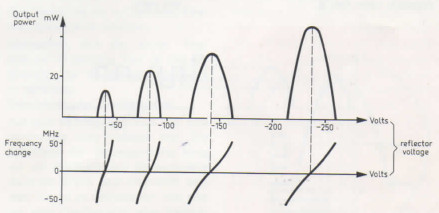
\includegraphics[width=0.7\textwidth]{pics/voltage_graphic.jpg}
                \caption{
                    In der Abbildungen sind 2 Graphen abgebildet. Der obere 
                    Graph zeigt den Verlauf der Reflektorspannung gegen die Ausgangsleistung von den
                    Mikrowellen vom Reflexklystron an. Die untere Graphik stellt parallel dazu
                    den Verlauf der Reflexionspannung gegen die Schwingungsfrequenz dar.\cite{Mikro}
                }
                \label{fig:2}
            \end{figure}
            Zur Abstimmung der Frequenz kommen zwei Prinzipien in Frage: 
            \begin{itemize}
               \item Das Ändern des Innendurchmessers des Hohlraumresonators (mechanische Abstimmung) 
               \item Das Verändern der Reflektorspannung (elektronische Abstimmung).
            \end{itemize}
        \subsection{Messung von Mikrowellen}
            Die Wellenlänge einer Mikrowelle kann mit einem Stehwellendetektor bestimmt werden.
            Dieser ist ein Hohlleiter mit einer Öffnung in der eine Sonde eingelassen ist, welche an ein SWR-Meter angeschlossen ist.
            Der doppelte Abstand zweier aufeinanderfolgender Minima einer stehenden Welle entspricht dabei der Hohlleiter-Wellenlänge $\lambda _g$. Die Frequenz $f$
            ergibt sich rechnerisch aus
            \begin{align}
                f &= c \sqrt{\left(\frac{1}{\lambda _g}\right)^2+\left(\frac{1}{2a}\right)^2} \label{eq:1}. \text{\cite{Mikro}}
            \end{align}
            Für die Messung der Hohlleiterwellenlänge muss sich in dem Hohlleiter eine stehende Welle der Mode $\text{TE}_{1,0}$ , der Grundmode, bilden.
            Diese ist die einzige Mode, über welche Mikrowellen in diesem Versuch ($f \approx \SI{9}{\giga\hertz}$) transportiert werden kann.
            Als Beispiel werden die Grenzwellenlängen für die Moden $\text{TE}_{1,0}$, $\text{TE}_{2,0}$ und $\text{TE}_{3,0}$ mit Gleichung \eqref{eq:G} berechnet:
            \begin{align}
                \lambda _{G,\text{TE}_{0,1}} &= \text{\input{lambda_g_1.tex}} \\
                \lambda _{G,\text{TE}_{0,2}} &= \text{\input{lambda_g_2.tex}} \\
                \lambda _{G,\text{TE}_{0,3}} &= \text{\input{lambda_g_3.tex}}.
            \end{align}
            Für die Breite des Hohlleiters ist der im Aufbau angegebene Wert verwendet worden. 


        \subsection{Stehwellenverhältnis (SWR)}
            Bei elektronischen Bauelementen kommt es an den Übergängen der Leitungen zu
            Reflexionen aufgrund von Unstetigkeiten in den Impedanzen. Diese Unstetigkeiten werden Fehlanpassungen genannt.
            Diese werden in Leitungen häufig versucht zu minimieren, um Verluste in der Leitung zu vermeiden.
            Das SWR oder auch die Welligkeit ist ein Maß für die Fehlanpassung. Ideale Anpassung entspricht SWR $= 1,0$, maximale Fehlanpassung SWR gegen Unendlich.
            
            Ein Gleitschraubentransformator kann genutzt werden, um den Hohlleiter zu einer gegebenen und unveränderlichen Impedanz anzupassen.\\
            Das SWR kann über verschiedene Methoden bestimmt werden, wobei drei von diesen in Abschnitt \ref{ssec:4.3} beschrieben sind.

%
% -- Aufbau -- %
%
    \section{Aufbau}
        Prinzipiell werden in diesem Versuch 12 verschiedene Bauteile verwendet:
        \begin{itemize}
            \item Klystron Netzteil
            \item Klystron
            \item Einweggleichrichter
            \item Frequenzmessgerät
            \item Dämpfungsglied
            \item Stehwellendetektor
            \item Abschluss
            \item verstellbarer Kurzschluss
            \item Gleitschraubentransformator
            \item Abgeschlossener Hohlleiter mit Diodendetektor
            \item SWR-Meter
            \item Oszilloskop
        \end{itemize}

        Die Beschleunigungs- und Reflektorspannungen, sowie die Modulationsspannung, welche am Klystron anliegen, werden durch das Klystron-Netzteil produziert.

        Der Einweggleichrichter ist essenziell und muss daher in jedem Versuchsaufbau direkt hinter dem Ausgang des Klystrons verbaut werden.
        Die aus dem Klystron austretenden Mikrowellen können nämlich theoretisch reflektiert werden und das Klystron zerstören.
        Durch den Einweggleichrichter wird dies verhindert, da dieser nur Elektromagnetische Wellen in eine Richtung durchlässt.

        \subsection{Modenmessung}
        Eine schematische Darstellung des Versuchsaufbaus ist in Abbildung \ref{fig:3} zu erkennen.
        Um nun die Moden des Klystrons zu messen muss hinter dem Dämpfungsglied zunächst ein Diodendetektor montiert werden.
        Nun wird ein Kanal des Oszilloskops mit dem Ausgang \enquote{0-30 V, 50 Hz} des Netzteils und der zweite Kanal mit dem Ausgang des Diodendetektors verbunden.
        \begin{figure}[H]
            \centering
            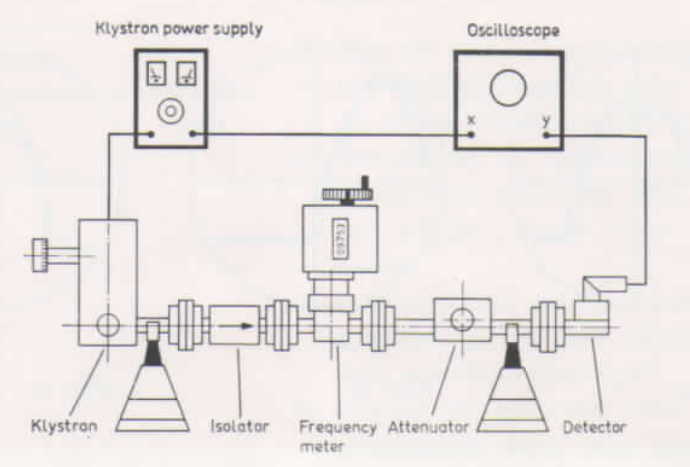
\includegraphics[width=0.7\textwidth]{pics/v53_1.png}
            \caption{Schematischer Aufbau für die Untersuchung der Moden und der elektronischen Abstimmung des Klystrons. Es sind hier die verwendeten Komponenten gezeigt und betitelt, sowie grob die Verkabelung der Komponenten mit den Netz- und Messgeräten dargestellt.\cite{Mikro}}
            \label{fig:3}
        \end{figure}

        \subsection{Messung von Frequenz, Wellenlänge und Dämpfung \label{ssec:3.2}}
        \begin{figure}[H]
            \centering
            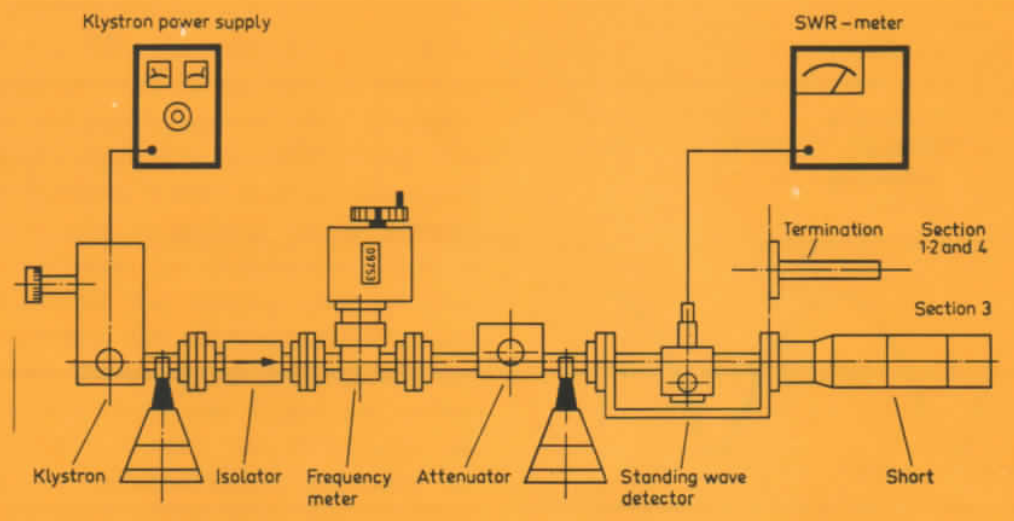
\includegraphics[width=0.8\textwidth]{pics/v53_2.png}
            \caption{Schematischer Aufbau für die Messung der Frequenz, Wellenlänge und Dämpfung. Es sind hier die verwendeten Komponenten gezeigt und betitelt, sowie grob die Verkabelung der Komponenten mit den Netz- und Messgeräten dargestellt.\cite{Mikro}}
            \label{fig:4}
        \end{figure}
        Eine schematische Darstellung des Versuchsaufbaus ist in Abbildung \ref{fig:4} zu erkennen.
        Für diese Messreihe muss zunächst das Oszilloskop vom Klystron-Netzteil und dem Detektor entfernt werden.
        Anstelle des Diodendetektors wird hinter dem Dämpfungsglied der Stehwellendetektor eingebaut.
        Hinter diesem wird nun entweder der Abschluss oder der Kurzschluss montiert, näheres hierzu wird in der Durchführung zu diesem Versuchsteil (Abschnitt \ref{ssec:4.2}) erklärt.
        Als letztes wird das SWR-Meter am Detektor des Stehwellenmessgeräts angeschlossen.

        \subsection{Messung des Stehwellenverhältnis \label{ssec:3.3}}
        Eine schematische Darstellung des Versuchsaufbaus ist in Abbildung \ref{fig:5} zu erkennen.
        Zunächst wird zwischen Abschluss und Stehwellendetektor der Gleitschraubentransformator eingesetzt.
        Der Rest des Aufbaus ist identisch.
        \begin{figure}[H]
            \centering
            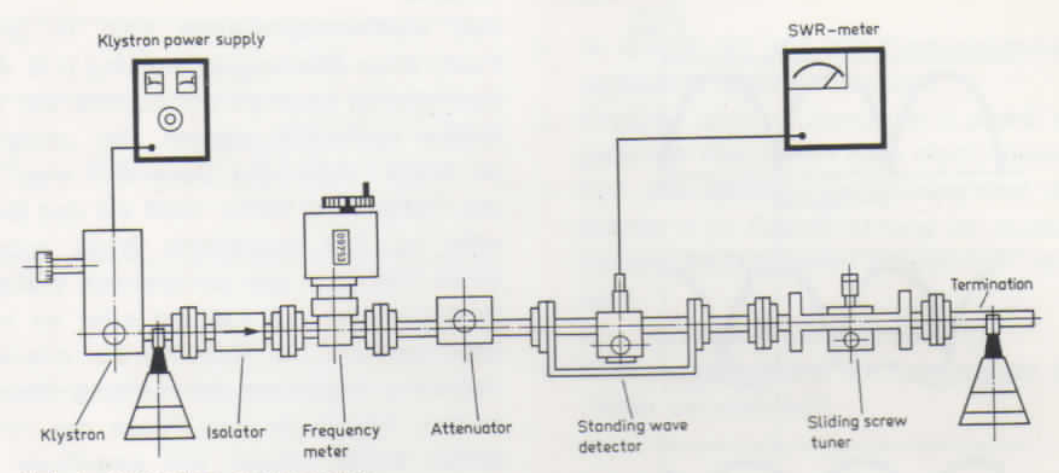
\includegraphics[width=0.8\textwidth]{pics/v53_3.png}
            \caption{Schematischer Aufbau für die Messung des Stehwellenverhältnis. Es sind hier die verwendeten Komponenten gezeigt und betitelt, sowie grob die Verkabelung der Komponenten mit den Netz- und Messgeräten dargestellt.\cite{Mikro}}
            \label{fig:5}
        \end{figure}
%
% -- Durchführung -- %
%
    \section{Durchführung}
        Zu Beginn der Durchführung des Versuches wird das Klystron etwa eine Minute angeschaltet und vorgeheizt.
        Hierzu wird das Netzteil angeschaltet und der \enquote{Res./Ref.}-Knopf zunächst ausgeschaltet.
        \subsection{Modenmessung}
            In diesem Versuchsteil werden sowohl die Moden, als auch die elektronische Abstimmung des Klystrons untersucht.
            
            Hierzu wird zunächst das Dämpfungsglied auf eine Dämpfung von $\SI{30}{\decibel}$ eingestellt und beim Oszilloskop der Kanal, welcher an das Netzteil angeschlossen ist auf die x-Ablenkung des Oszilloskops gesetzt, und der Kanal, welcher an dem Detektor angeschlossen ist auf die y-Ablenkung gesetzt.
            Die vorläufigen Ablenkkoeffizienten werden zunächst auf $10\symup{mV/Teil}$ für die x-Ablekung und $10\symup{V/Teil}$ für die y-Achse gestellt.

            Nun wird der Knopf \enquote{50 Hz} auf dem Netzteil gedrückt, der Knopf \enquote{Res/Refl. on} in die \textit{Aus} Position gestellt und der Drehregler für die Reflektorspannung in Mittellage gestellt.
            Die horizontale Linie auf dem Oszilloskop wird nun symmetrisch zur vertikalen Mittellinie gesetzt.
            Nun wird der Knopf \enquote{Res./Refl. on} in die \textit{Ein} Position gebracht und zunächst eine Reflektorspannung von ca. $\SI{200}{\volt}$ eingestellt.
            Die Reflektorspannung und das Oszilloskop werden nun umgestellt bis ein Modus wie in Abbildung \ref{fig:6} zu erkennen ist.

            \begin{figure}[H]
                \centering
                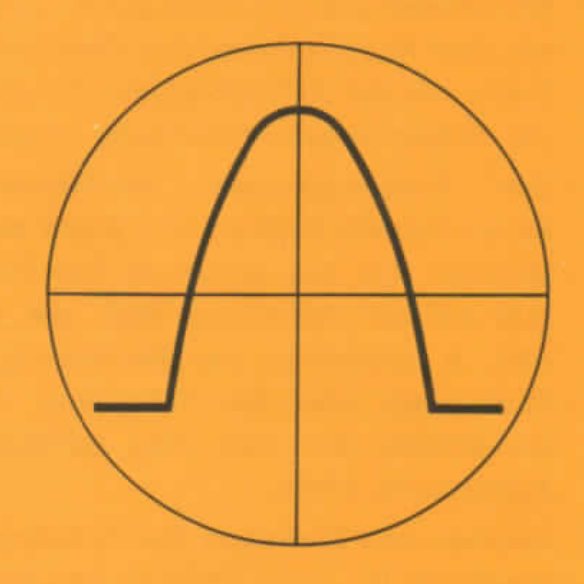
\includegraphics[width=0.5\textwidth]{pics/modus.png}
                \caption{Beispielhafte Abbildung der Modenkurve eines Klystrons.\cite{Mikro}}
                \label{fig:6}
            \end{figure}

            Nun wird der Frequenzmesser auf das Maximum des Modus abgestimmt.
            Dies ist an einem dip in der Amplitude des Modus zu erkennen, welcher sich dann in der Mitte des Modus abbilden sollte.
            Die Mittelfrequenz des Modus wird dann am Frequenzmesser abgelesen.
            Nun wird der Frequenzmesser verstimmt und dann werden die Reflektorspannung am Netzteil und Amplitude am Oszilloskop aufgenommen.
            
            Das Ablesen der Frequenz/Amplitude/Reflektorspannung wird nun für die Enden des Modus wiederholt und der gesamte Prozess zum Messen des Maximum und der Enden für zwei weitere Moden bei kleineren Reflektorspannungen wiederholt.

            Für die elektronische Abstimmung wird die Reflektorspannung auf den höchsten Modus gesetzt.
            Es werden nun die Frequenz und die Reflektorspannung für die Punkte halber Leistung an beiden Enden des Modus gemessen.
            Eine Abbildung, welche die korrekte Durchführung dieses Verfahrens beschreibt ist in Abbildung \ref{fig:7} zu erkennen.
            \begin{figure}[H]
                \centering
                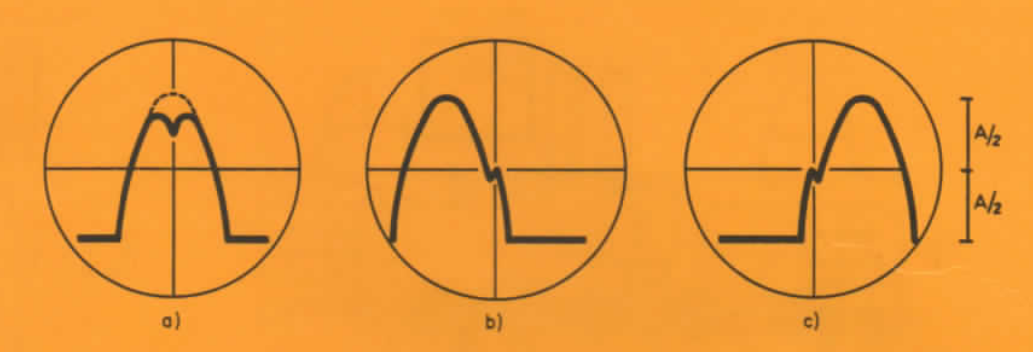
\includegraphics[width=0.7\textwidth]{pics/abstimmung.png}
                \caption{Hier abgebildet sind schematische Darstellungen der Modenkurven bei der Messung der elektronischen Abstimmung. Die Messung der Frequenz und Reflektorspannung wird an der Spitze des Modus in a), sowie an den beiden Punkten halber Leistung b) und c) durchgeführt.\cite{Mikro}}
                \label{fig:7}
            \end{figure}

        \subsection{Messung von Frequenz, Wellenlänge und Dämpfung \label{ssec:4.2}}
            Für diesen Versuchsteil wird zuerst der \textbf{Versuchsaufbau} wie in \ref{ssec:3.2} aufgebaut, wobei zunächst der Abschluss an das Ende des Aufbaus montiert wird.
            Der Abschluss absorbiert die Strahlung vollständig und verhindert damit Reflexion.
            Es wird außerdem das Dämpfungsglied auf $\SI{20}{\decibel}$ und die Sondentiefe beim Stehwellendetektor  auf die rote Markierung eingestellt.

            Das \textbf{SWR-Meter} wird auf $\SI{40}{\decibel}$ mit einer Bandbreite von $\SI{100}{\hertz}$ gestellt und die Drehschalter für $\SI{1}{\kilo\hertz}$ und Verstärkung werden in Mittelstellung gebracht.
            Der $\SI{1}{\kilo\hertz}$-Schalter muss während der Durchführung der Versuche unbedingt nicht aus der Mittelstellung gebracht werden.
            
            Nun wird \textbf{beim Klystron} die $\SI{1}{\kilo\hertz}$-Rechteck-Modulation angeschaltet und der Modus bei ca. $\SI{200}{\volt}$ eingestellt.
            Als letztes wird nun die Reflektorspannung so eingestellt, dass sich am SWR-Meter ein Maximum einstellt.
            Es muss dabei möglicherweise der $\si{\decibel}$-Bereich umgestellt werden, damit der Ausschlag in der Skala bleibt.

            \subsubsection{Frequenzmessung}
                Für die Messung der Frequenz wird der Frequenzmesser eingestellt, bis der Ausschlag am SWR-Meter sinkt.
                Die Frequenz beim minimalen Ausschlag wird abgelesen und notiert.
                
            \subsubsection{Wellenlängenmessung\label{sssec:4.2.2}}
                Als nächstes wird die Wellenlänge gemessen.
                Hierzu wird der Abschluss mit dem Kurzschluss ausgetauscht und der Frequenzmesser zunächst wieder verstimmt.
                Der Kurzschluss sorgt dafür, dass die eintreffende Strahlung fast vollständig reflektiert wird und sich somit im Hohlleiter eine stehende Welle ausbildet.
                
                Nun wird am Stehwellendetektor die Sonde solange verschoben, bis sich ein Minimum am SWR-Meter einstellt.
                Es wird dann die Distanz der Sonde bei diesem und dem darauffolgenden Minimum abgelesen und notiert.
                
                Die Innenabmessung des Hohlleiters ist gegeben als $\SI{22.860(46)}{\milli\meter}$ \cite{Mikro} .

            \subsubsection{Dämpfungsmessung}
                Zuletzt soll die Dämpfung durch das Dämpfungsglied gemessen werden.
                Hierzu wird der Kurzschluss erneut mit dem Abschluss ausgetauscht.
                
                Bei dem SWR-Meter soll nun zunächst im $\SI{30}{\decibel}$-Bereich ein Vollausschlag ($0$ auf der $\si{\decibel}$-Skala) erreicht werden, wobei dies zunächst durch einstellen der Verstärkung und wenn nötig noch mit der Einstellung des Dämpfungsglieds erreicht wird.
                Hierfür wird dann die Einstellung der Mikrometerschraube und die daraus aus der Eichkurve resultierende Dämpfung abgelesen und eingetragen.
                
                Nun wird die Mikrometerschraube wiederholt gedreht, sodass sich $\SI{2}{\decibel}$-Schritte auf der Skala des SWR-Meters ergeben, und für jeden Schritt erneut wie zuvor gemessen.
                Dies wird bis zu einem Ausschlag am SWR-Meter von $\SI{10}{\decibel}$ durchgeführt.

        \subsection{Messung des Stehwellenverhältnis \label{ssec:4.3}}
            Zuerst wird der Aufbau wie in Abschnitt \ref{ssec:3.3} aufgebaut.
            Das Dämpfungsglied wird hier zunächst auf eine Dämpfung von $\SI{20}{\decibel}$ eingestellt und das SWR-Meter in den $\SI{40}{\decibel}$-Bereich mit einer Bandbreite von $\SI{20}{\hertz}$ gebracht.
            
            Am Gleitschraubentransformator wird die Sonde auf $\SI{0}{\milli\meter}$ herausgedreht und am Stehwellenmessgerät sichergestellt, dass die Sonde auf der roten Markierung steht.
            Die Einstellungen des Klystrons sind hier zunächst die gleichen wie in Abschnitt \ref{ssec:4.2}.
            Am SWR-Meter wird ein mittlerer Ausschlag eingestellt.
            \subsubsection{Direkte Messung mit SWR-Meter}
                Bei der direkten Messung wird das SWR
                über ein SWR-Meter, welches an den Stehwellendetektor angeschlossen ist, direkt gemessen.
                Diese Methode kann für kleine und mittlere SWR angewendet werden.

                Für kleine Sondentiefen ist das SWR direkt mit dem SWR-Meter einfach und genau messbar.
                Hierzu wird die Sonde des Gleitschraubentransformators zunächst auf $\SI{5}{\milli\meter}$ eingestellt.
                
                Die Sonde des Stehwellendetektors wird nun zu einem Maximum am SWR-Meter gebracht und die Verstärkung so eingestellt, dass auf der SWR-Skala ein Wert von $\num{1.0}$ einstellt.
                Nun wird die Sonde ohne Veränderung an den SWR-Meter Einstellungen verschoben bis sich ein Minimum im Ausschlag ergibt, welches dann abgelesen und notiert wird.
                
                Diese Messungen werden dann für Sondeneinstellungen des Gleitschraubentransformators von $3$, $7$ und $\SI{9}{\milli\meter}$ erneut durchgeführt.
                
            \subsubsection{3dB-Methode}
                Das Messen starker Welligkeiten erfordert tieferes Einbringen der Messsonde, was zu Feldverzerrungen und hohen Leistungen am Detektor führt, wodurch dieser
                nicht in seinem vorgesehenem Arbeitsbereich misst.
                Um dies zu umgehen wird die \enquote{$\SI{3}{\decibel}$-Methode} angewendet.
                Dafür wird der Abstand zwischen zwei Punkten gemessen, wo die Ausgangsspannung am Detektor 
                einen Faktor zwei vom Minimum erzielt. Das SWR $S$ ergibt sich dann über die Formel
                \begin{align}
                    S &= \sqrt{1+\frac{1}{\sin ^2 \frac{\pi (d_1-d_2)}{\lambda_g}}} \label{eq:2}, \text{\cite{Mikro}}
                \end{align}
                Hier beschreibt $d_{1,2}$ die Schlittenstellung am Hohlleiter an einem Vollausschlag im SWR-Meter links und rechts vom Minimum.
            
                Zunächst wird die Sondentiefe am Gleitschraubentransformator auf $\SI{9}{\milli\metre}$ eingestellt.
                Mit dem Stehwellendetektor wird dann die Sonde in einen minimalen Ausschlag am SWR-Meter gebracht und die Verstärkung auf einen Ausschlag auf der $\si{\decibel}$-Skala von $\SI{3}{\decibel}$ eingestellt.
                
                Nun wird die Sonde des Stehwellendetektors in eine Richtung verschoben, bis sich ein Vollausschlag (also $\SI{0}{\decibel}$) ergibt.
                Hier wird nun die Schlittenstellung notiert und der Prozess für das Verschieben in die andere Richtung widerholt.

                Nun wird der Gleitschraubentransformator auf 0 gestellt und der Abschluss mit dem Kurzschluss ersetzt, wonach der Abstand zwischen zwei aufeinanderfolgenden Minima wie in Abschnitt \ref{sssec:4.2.2} gemessen wird.
                
            \subsubsection{Abschwächer-Methode}
                Bei einem SWR von größer als 10 wird die \enquote{Abschwächer-Methode} verwendet.
                Hierbei wird ein Abschwächer genutzt, welcher das Ausgangssignal vom Maximum und Minimum angleicht. 
                Mit der Einstellung des Abschwächers $(A_2-A_1) $ wird dann das SWR berechnet
                \begin{align}
                    A_2-A_1 = 20 \log S \label{eq:3}. \text{\cite{Mikro}}
                \end{align}
                Dabei beschreibt $A_{1,2}$ die Einstellung des Dämpfungsglieds, an den Stellungen, wo die beiden Signale vom Minimum und Maximum gleich werden.
            
                Die Sonde des Gleitschraubentransformators wird zuerst wieder auf $\SI{9}{\milli\metre}$ gestellt und die Sonde des Stehwellendetektors in ein Minimum des SWR-Meters gebracht.
                Nun wird überprüft, dass das Dämpfungsglied auf einer Dämpfung von $\SI{20}{\decibel}$ steht.

                Die Verstärkung des SWR-Meters wird nun erst auf einen Ausschlag von $\SI{3}{\decibel}$ verschoben, dann wird die Sonde des Stehwellendetektors verschoben und das Dämpfungsglied dabei so umgestellt, dass der Ausschlag des SWR-Meters nicht die Skala verlässt.
                Auf diese Weise muss ein relatives Maximum gefunden werden und dann das Dämpfungsglied so eingestellt werden, dass sich wieder ein Ausschlag von $\SI{3}{\decibel}$ ergibt.
                
                Die Einstellung des Dämpfungsglieds nun ablesen und notieren.
%
% -- Auswertung -- %
%
    \section{Auswertung}
        Alle Berechnungen und Fehler sind in der Auswertung mit scipy \cite{scipy}, numpy \cite{numpy} und
        uncertainties \cite{uncertainties} durchgeführt worden.
            \subsection{Modenmessung}
                Die Messwerte für die Modenmessung sind in Tabelle \ref{tab:1} gegeben.
                \begin{table}[H]
                    \centering
                    \caption{
                        In der Tabelle sind die Messwerte für die Modenmessung eingetragen.
                        Die verschiedenen Moden entsprechen den Moden aus Abbildung \ref{fig:2}, bei
                        welchem jeweils die Reflektorspannung $U_0$ gegen die Amplitude und Resonanzfrequenz der Mode, sowie
                        der Reflektorspannungen $U_1$ und $U_2$ der Schnittpunkte mit der x-Achse.
                    } 
                    \input{table_moden.tex}
                    \label{tab:1} 
                \end{table}
                
                Der Plot der Messwerte für die einzelnen Moden des Reflexklystrons ist in der folgenden Abbildung \ref{fig:8}  zu sehen.

                \begin{figure}[H]
                    \centering
                    \includegraphics[width=\textwidth]{build/moden.pdf}
                    \caption{
                        In der Abbildung sind die Moden des Reflexklystrons, welche aus den Daten
                        der Tabelle \ref{tab:1} rekonstruiert worden sind zu sehen. Aufgetragen ist 
                        hierbei die Reflektorspannung gegen die am Oszilloskop gemessenene Spannung. Insgesamt sind die Messwerte von drei
                        Moden sowie deren Fits aufgetragen.
                    }
                    \label{fig:8}
                \end{figure}
                Die Fitkurven der einzelnen Moden sind dabei mit der Fitfunktion
                \begin{align}
                    y = a x^2 + b x + c
                \end{align}
                geplottet worden. Die Fitparameter der einzelnen Moden sind dabei gegeben als
                \begin{align}
                    a_{1.Mode} &= \text{\input{a_U1}}\\
                    b_{1.Mode} &= \text{\input{b_U1}}\\
                    c_{1.Mode} &= \text{\input{c_U1}}\\
                    a_{2.Mode} &= \text{\input{a_U2}}\\
                    b_{2.Mode} &= \text{\input{b_U2}}\\
                    c_{2.Mode} &= \text{\input{c_U2}}\\
                    a_{3.Mode} &= \text{\input{a_U3}}\\
                    b_{3.Mode} &= \text{\input{b_U3}}\\
                    c_{3.Mode} &= \text{\input{c_U3}}.
                \end{align}

                Die Messwerte für die elektronische Abstimmung sind in der folgenden Tabelle \ref{tab:2} gegeben.
                \begin{table}[H]
                    \centering
                    \caption{
                        In der Tabelle sind die Messwerte für die elektronische
                        Abstimmung eingetragen. Dabei werden für die Punkte halber Leistung wie in Abbildung
                        \ref{fig:7} die Reflektionsspannung und die dazugehörige Resonanzfrequenz bestimmt.\cite{matplotlib}
                    } 
                    \input{table_abstimmung.tex}
                    \label{tab:2}
                \end{table}
                Mit diesen wird die elektronische Bandbreite und die Abstimmempfindlichkeit bestimmt.
                Die elektronische Bandbreite ist dabei definiert als
                \begin{align}
                    \abs{f'-f''} &= \text{\input{f_breite.tex}} \text{\cite{Mikro}} \label{eq:14}
                    \intertext{
                        und die elektronische Abstimmung ist definiert als
                    }
                    \frac{f'-f''}{V'-V''} &= \text{\input{abstimm.tex}} \text{\cite{Mikro}} \label{eq:15}
                \end{align}
                Dabei stehen die Teilstriche für die Punkte halber Leistung, $f$ für die Frequenz und $V$ für die Reflektorspannung.

            \subsection{Messung von Frequenz, Wellenlänge und Dämpfung} \label{ssec:5.2}
                Die Messwerte für die Messung der Frequenz und der Wellenlänge sind in der
                nachfolgenden Tabelle \ref{tab:3} eingetragen.
                \begin{table}[H]
                    \centering
                    \caption{
                        Messwerte für die Messung der Resonanzfrequenz des Reflexklystrons $f_{\text{Res}}$ und Hohlleiterwellenlänge $\lambda_g$
                        sowie der Mikrowellenfrequenz $f_{\text{mik}}$.
                        Gemessen worden ist dabei die Resonanzfrequenz $f_{\text{Res}}$ sowie die Position der beiden Minima des SWR auf der Messleitung des Hohlleiters.
                        $\lambda_g$ entspricht dabei der doppelten betragsmäßigen Differenz der beiden Minima.
                        Die Mikrowellenfrequenz ist dabei mit Gleichung \eqref{eq:1} und der gegebenen
                        Innenabmessung des Hohlleiters a \cite{Mikro} berechnet worden.
                    }
                    \input{table_frequenz.tex}
                    \label{tab:3} 
                \end{table}  
                Die Hohlleiterwellenlänge ist dabei aus der doppelten, betragsmäßigen Differenz der beiden Minima
                berechnet worden. Die Frequenz der Mikrowelle $f_{\text{mik}}$ ist mit den Messwerten
                aus der Tabelle \ref{tab:3} und der Gleichung \eqref{eq:1} ermittelt worden.\\


                Die Messwerte für die Dämpfung sind in der folgenden Tabelle \ref{tab:4} aufgetragen.
                \begin{table}[H]
                    \centering
                    \caption{
                        Messwerte für die Dämpfung.
                        Gemessen worden ist der Ausschlag am SWR-Meter gegen die Mikrometereinstellung
                        des Dämpfungsglieds. Die Dämpfung ist mithilfe eines Graphen auf dem Dämpfungsglied,
                        welches den Zusammenhang zwischen Mikrometereinstellung und Dämpfung aufzeigt, ermittelt worden.
                    } 
                    \input{table_daempfung.tex}
                    \label{tab:4}
                \end{table}
                Nun kann die mit dem SWR-Meter gemessene Dämpfung mit der durch das Dämpfungsglied verursachte Dämpfung welche an der Eichkurve abgelesen wurde verglichen werden.
                
                Hierzu wurden die Werte zu den beiden zuvor genannten Dämpfungen gegen die Schraubenstellung des Dämpfungsglieds aufgetragen.
                Es werden außerdem Fits an die beiden Datensätze durchgeführt um die Eichkurve und die aus der Messung mit dem SWR-Meter erhaltene Kurve vergleichen zu können.
                Dies ist in Abbildung \ref{fig:9} zu erkennen.
                \begin{figure}[H]
                    \centering
                    \includegraphics[width=\textwidth]{build/Dämpfung.pdf}
                    \caption{
                        Eine Abbildung der gemessenen Schraubenstellung in $\si{\milli\meter}$ gegen die Dämpfung in $\si{\decibel}$.
                        Eingetragen sind zum einen die Messdaten für die Dämpfung, welche mit dem SWR-Meter gemessen wurden, und zum anderen jene, die aus der Eichkurve des Dämpfungsglieds abgelesen wurden.
                        Außerdem sind die berechneten Fitkurven eingetragen. \cite{matplotlib}
                    }
                    \label{fig:9}
                \end{figure}
                
                Die Fits wurden mit einer Fitfunktion der Form
                \begin{equation}
                    y = 10^{ax} + b \label{eq:16}
                \end{equation}
                Wobei $y$ hier die Dämpfung ist, $x$ die Schraubenstellung, und $a$ und $b$ die Fitparameter welche die Krümmung der Kurve und den y-Achsenabschnitt der Kurve bestimmen.
                Es ergeben sich hiermit die Fitparameter
                \begin{align}
                    a_{SWR} &= \input{build/a1.tex} \label{eq:17}\\
                    b_{SWR} &= \input{build/b1.tex}\\
                    \intertext{für die Messungen der Dämpfung mit dem SWR-Meter und}
                    a_{Eich} &= \input{build/a2.tex}\\
                    b_{Eich} &= \input{build/b2.tex} \label{eq:20}
                \end{align}
                für die Werte aus der Eichkurve.

            
            \subsection{Messung des Stehwellenverhältnis}
                \subsubsection{Direkte Messung mit SWR-Meter}
                    Die Messwerte für die direkte Messung mit einem SWR-Meter sind in der nachfolgenden Tabelle \ref{tab:5}
                    eingetragen.
                    \begin{table}[H]
                        \centering
                        \caption{
                            Messwerte der direkten Messung mit dem SWR-Meter.
                            Hierbei ist die Sondentiefe am Gleitschraubentransformator gegen
                            das SWR gemessen worden.
                        } 
                        \input{table_methode1.tex}
                        \label{tab:5}
                    \end{table}

                \subsubsection{3dB-Methode}
                    Die Messwerte für die Messung des SWR mit der 3dB-Methode sind in der folgenden Tabelle \ref{tab:6} gegeben.
                    \begin{table}[H]
                        \centering
                        \caption{
                            Messwerte für die Messung des SWR mit der 3dB-Methode.
                            Gemessen worden sind die Schlittenstellung $d_1$ und $d_2$ zweier benachbarter Vollausschläge im SWR, sowie dem Abstand zweier aufeinanderfolgender
                            Minima. Die Hohlleiterwellenlänge entspicht dabei der doppelten betragsmäßigen Differenz der beiden Minima. Das SWR ist dabei mit Gleichung
                            \eqref{eq:2} berechnet worden.
                        }
                        \input{table_methode2.tex}
                        \label{tab:6} 
                    \end{table}
                    Die Hohlleiterwellenlänge wird dabei wie in Abschnitt \ref{ssec:5.2} berechnet.
                    Das SWR wird dabei mithilfe der Gleichung \eqref{eq:2} berechnet.


                \subsubsection{Abschwächer-Methode}
                    Die Messwerte für die Bestimmung des SWR mit der Abschwächer-Methode sind in der Tabelle \ref{tab:7} eingetragen.
                        \begin{table}[H]
                            \centering
                            \caption{
                                Messwerte des SWR mit der Abschwächer Methode.
                                Gemessen worden sind dabei die Einstellungen des Dämpfungsglied $A_1$ und $A_2$, an den Stellungen,
                                wo die beiden Signale vom Minimum und Maximum gleich werden. Das SWR ist mit Gleichung \eqref{eq:6} berechnet worden.
                            }
                            \input{table_methode3.tex}
                            \label{tab:7} 
                        \end{table} 
                        Das SWR ist nach dem Umstellen mit der Gleichung \eqref{eq:3} berechnet worden.
                        Die umgestellte Formel lautet dann
                        \begin{align}
                            S = 10^{\frac{A_2-A_1}{20}}. \label{eq:6}
                        \end{align}

%
% -- Diskussion -- %
%
    \section{Diskussion}
        
        \subsection{Modenmessung}
            Bei der Modenmessung fällt zunächst auf, wie in Abbildung \ref{fig:8} zu erkennen, dass die Maxima der Moden im Vergleich mit der Modenkurve in Abbildung \ref{fig:2} nicht bei abnehmender Reflektorspannnung quasi-linear in ihrer Amplitude abfallen, sondern der erste gemessene Modus, bei welchem die maximale Amplitude der Moden erwartet ist, eine kleinere Amplitude als der darauffolgende hat.\newline
            Dabei ist jedoch auch zu bemerken, dass das gemessene Maximum des 2. Modus nicht mit dem Maximum der Fitparabel übereinstimmt, was das Maximum in der Fitkurve deutlich höher ausfallen lässt, als den gemessenen Wert.
            \newline
            Es kann hier sein, dass ein Fehler entweder in der Messung der Reflektorspannung bei Maximalamplitude oder bei einem oder beiden Enden des Modus aufgetreten ist, welcher dies erklären würde.
            Dies würde den Unterschied in der Höhe der Moden deutlich verringern, jedoch ist auch der gemessene Wert der maximalen Amplitude des zweiten Modus auch noch leicht größer als der des Ersten.
            \newline
            Der Abfall der Modenbreite bei geringerer Reflektorspannung ist wiederum in der Messung konsistent mit der in Abbildung \ref{fig:2} zu erkennenden.
            
            Bei der elektronischen Abstimmung wurde der zweite Modus vermessen, da hier die größte Maximalamplitude gemessen wurde.
            Es ergibt sich eine elektronische Bandbreite von  $\input{build/f_breite.tex}$  und eine Abstimm-Empfindlichkeit von $\input{build/abstimm.tex}$s, wie in Gleichungen \eqref{eq:14} und \eqref{eq:15} berechnet.
            Die elektronische Bandbreite ist ein Maß für den Frequenzbereich in dem das Klystron allein durch elektische Abstimmung effizient arbeitet und ist in diesem Fall im vergleich zu der Frequenz mit der das Klystron betrieben wird äußerst gering.
            Jedoch ergibt sich damit eine hohe Abstimm-Empfindlichkeit, was dazu führt, dass die elektronischer Abstimmung eine relativ zur Betriebsfrequenz genaue Einstellung der Frequenz erlaubt.

        \subsection{Messung von Frequenz, Wellenlänge und Dämpfung}
            \subsubsection{Frequenz- und Wellenlängenmessung\label{sssec:6.2.1}}
                Die Messung der Frequenz direkt mit dem Frequenzmessgerät $f_{\symup{Res}}$, sowie die Hohlleiterwellenlänge $\lambda_g$ und die aus dieser berechnete Frequenz $f_{\symup{mik}}$ ergibt die in Tabelle \ref{tab:3} eingetragenen Werte.
                Hier wird deutlich, dass die mit dem Frequenzmesser bestimmte Frequenz und die durch die Wellenlängenmessung berechnete Frequenz fast identisch sind, und die Abweichung leicht mit der Unsicherheit aufgrund der Abweichung des Innendurchmessers des Hohlleiters erklärt werden kann.
                
                Mithilfe der Hohleiterwellenlänge und der Mikrowellenfrequenz aus Tabelle \ref{tab:3} kann die Phasengeschwindigkeit der
                Mikrowelle über das Produkt berechnet werden. Diese ergibt sich, in Einheiten der 
                Lichtgeschwindigkeit, zu 
                \begin{align}
                    v_{\text{Phase}} &= \text{\input{v_phase.tex}}.
                \end{align}
                Die Phasengeschwindigkeit ist hierbei größer als die Lichtgeschwindigkeit, was physikalisch
                gesehen aber unproblematisch ist, da die Phasengeschwindigkeit keine Informationen transportiert.
                Informationen werden durch die Gruppengeschwindigeit transportiert, welche kleiner als die Lichtgeschwindigkeit ist.
            \subsubsection{Dämpfung}
                In Abbildung \ref{fig:9} sind die für diesen Versuchsteil relevanten Messdaten und Fitkurven eingetragen.
                Von Bedeutung sind hier die berechneten Fitparameter der Kurven, besonders dabei der Fitparameter $a$, da dieser entscheidend ist für die Krümmung der Kurve, während Parameter $b$ nur eine relativ unwichtige y-Achsenverschiebung erzeugt.

                Diese Fitparameter sind in Gleichungen \eqref{eq:17} bis \eqref{eq:20} eingetragen.
                Vergleicht man die Fitparameter $a$ der beiden Messungen ist sofort zu erkennen, dass diese fast identisch sind, was bedeutet, dass die Kurven bis auf die zuvor genannte y-Achsenverschiebung identisch sind.

                Hieraus lässt sich schließen, dass die gemessene Dämpfungskurve die gleiche Form hat wie die Eichkurve, was zum einen die Eichkurve validiert, und zum anderen darauf deutet, dass das Dämpfungsglied funktionstüchtig ist.
                Der Unterschied in der y-Achsenverschiebung der Kurven lässt sich damit begründen, dass die Skala des SWR-Meters nur Dämpfungen von $0-10\si{\decibel}$ wiedergeben kann, und daher eine Verstärkung des Signals notwendig war um die Messung auf die Skala zu bringen.
                
                Außerdem hat die Schraube am Dämpfungsglied einen Offset, was dazu führt, dass der abgelesene Wert der Schraubenstellung nicht der auf der Eichkurve entspricht.
                Deshalb kann der y-Achsenabschnitt des Eichkurvenfits mit einem einen Offset von etwa $\SI{3.2}{\milli\metre}$ korrigiert werden indem mit Formel \ref{eq:16} die Gleichung 
                \begin{align}
                    y_{Eich,Korrigiert}(x) &= 10^{a_{Eich}x} + b_{Eich,Korrigiert} \label{eq:23} \\    
                    b_{Eich,Korrigiert} &= b_{Eich} - y_{Eich}(3.2)\\
                \end{align}
                als korrigierte Eichkurve verwendet wird.
                
                Dies ist in Abbildung \ref{fig:10} gezeigt, wobei nun zu erkennen ist, dass der y-Achsenabschnitt der korrigierten Fitkurve $b_{Eich,Korrigiert} = \input{build/b_eich.tex}$ mit einem relativen Fehler zu $b_{SWR}$ von nur $\input{build/rf_eich.tex}$ jetzt deutlich besser zu dem des mit dem SWR-Meter gemessenen Daten passt.
                \begin{figure}[H]
                    \centering
                    \includegraphics[width=\textwidth]{build/Dämpfung_offset.pdf}
                    \caption{
                        Eine Abbildung der gemessenen Schraubenstellung in $\si{\milli\meter}$ gegen die Dämpfung in $\si{\decibel}$.
                        Eingetragen sind zum einen die Messdaten für die Dämpfung, welche mit dem SWR-Meter gemessen wurden, und zum anderen jene, die aus der Eichkurve des Dämpfungsglieds abgelesen wurden.
                        Außerdem sind die berechneten Fitkurven, sowie die korrigierte Eichkurve aus Gleichung \eqref{eq:23} eingetragen. \cite{matplotlib}
                    }
                    \label{fig:10}
                \end{figure}

        \subsection{Messung des Stehwellenverhältnis}
            \subsubsection{Direkte Messung mit SWR-Meter\label{sssec:6.3.1}}
                Für diese Messung sind die Messwerte in Tabelle \ref{tab:5} aufgenommen worden.
                Hierbei ist zu erkennen, dass das SWR bei kleinen Sondentiefen noch relativ gering ausfällt, aber bei hohen Sondentiefen deutlich größer wird, wobei bei großen Sondentiefen sogar ein SWR von $\infty$ erreicht wird.
                Es ist dabei anzumerken, dass die Messung mit dem SWR-Meter nur genau für kleine SWR ist.

                Bei großen Sondentiefen ist das SWR-Meter nicht mehr genau genug um annährend richtige Ergebnisse zu liefern, weshalb am Ende der Skala des SWR-Meters $\infty$ eingetragen ist, obwohl das SWR -- wie in den folgenden Messungen zu erkennen -- eigentlich einen endlichen Wert hat.
            
            \subsubsection{3dB-Methode \label{sssec:6.3.2}}
                In dieser Messreihe wurde die 3dB-Methode zur Messung großer SWR durchgeführt, und außerdem erneut die Hohlleiterwellenlänge gemessen, da diese für die Berechnung benötigt wird.
                
                Die gemessene Hohleiterwellenlänge stimmt gut mit der in Abschnitt \ref{sssec:6.2.1} diskutierten überein, wobei sich die geringe Abweichung durch Ablesefehler und Ungenauigkeit in der Bestimmung der Position des Minimums erklären lassen.

                Bei dem berechneten SWR ist zu erkennen, dass dieses deutlich größer ist als die endlichen Werte bei der direkten Bestimmung in Abschnitt \ref{sssec:6.3.1}, und für die gleiche Sondentiefe von $\SI{9}{\milli\meter}$ in dieser Messung eindeutig ungleich $\infty$ ist.
                Jedoch ergibt sich hier ein deutlich unterschiedlicher Wert als mit der Abschwächer-Methode, welche in Abschnitt \ref{sssec:6.3.3} diskutiert wird.
                Wieder der Erwartung, dass sich annährend gleiche Messwerte ergeben sollten, ergibt sich hier ein dramatischer Unterschied in den gemessenen SWR.
                
                Jedoch kann dies gut mit einem Ablesefehler bei der Position von $d_1$ und $d_2$ erklärt werden.
                Da diese sehr nahe beieinander liegen, führt die daraus resultierenden kleine Differenz in Kombination mit der Formel zur Berechnung \eqref{eq:2} schon bei kleinen Ablesefehlern zu großen Fehlern im SWR.

                Schon bei einem durchaus realistischen Ablesefehler von nur $\SI{1}{\milli\meter}$ ergibt sich ein SWR von $S = \input{build/SWR_2.tex}$, was mit Einbezug des Fehlers deutlich näher an dem in Abschnitt \ref{sssec:6.3.3} besprochenen SWR liegt.

            \subsubsection{Abschwächer-Methode \label{sssec:6.3.3}}
                Die Abschwächer Methode ist eine weitere Möglichkeit hohe SWR genau zu messen.
                Das gemessene SWR ist in Tabelle \ref{tab:7} eingetragen.

                Der bereits in Abschnitt \ref{sssec:6.3.2} behandelte Unterschied in den gemessenen SWR kann auch zum Teil mit einem Ablesefehler bei dieser Messung begründet werden.
                Aufgrund der Zehnerpotenz wird auch hier ein kleiner Ablesefehler zu relativ großen Abweichungen im SWR führen.
                Da das Ablesen der Dämpfung an der Eichkurve des Dämpfungsglieds auch nur begrenzt genau ist, wäre ein Ablesefehler von $\SI{2}{dB}$ durchaus möglich.
                Bei dieser Abweichung ergibt sich ein SWR von $S = \input{build/SWR_3.tex}$.

                Abschließend ist jedoch zu bemerken, dass SWR wie die hier gemessenen in der Anwendung bereits unvertretbar groß sind.
                Es wird in der Praxis mit SWR im Bereich von $\num{1.0} - \num{1.1}$ gearbeitet, wobei ein SWR $>3$ bereits eine unbrauchbare Fehlanpassung bedeutet, da der Verlust in der Leistung viel zu groß wird.
            
\newpage
\nocite{jannachexperimente}
\nocite{mikroschaden}
\printbibliography
\end{document}
